%% Creator: Inkscape inkscape 0.48.5, www.inkscape.org
%% PDF/EPS/PS + LaTeX output extension by Johan Engelen, 2010
%% Accompanies image file 'Rotsubrelerro.pdf' (pdf, eps, ps)
%%
%% To include the image in your LaTeX document, write
%%   \input{<filename>.pdf_tex}
%%  instead of
%%   \includegraphics{<filename>.pdf}
%% To scale the image, write
%%   \def\svgwidth{<desired width>}
%%   \input{<filename>.pdf_tex}
%%  instead of
%%   \includegraphics[width=<desired width>]{<filename>.pdf}
%%
%% Images with a different path to the parent latex file can
%% be accessed with the `import' package (which may need to be
%% installed) using
%%   \usepackage{import}
%% in the preamble, and then including the image with
%%   \import{<path to file>}{<filename>.pdf_tex}
%% Alternatively, one can specify
%%   \graphicspath{{<path to file>/}}
%% 
%% For more information, please see info/svg-inkscape on CTAN:
%%   http://tug.ctan.org/tex-archive/info/svg-inkscape
%%
\begingroup%
  \makeatletter%
  \providecommand\color[2][]{%
    \errmessage{(Inkscape) Color is used for the text in Inkscape, but the package 'color.sty' is not loaded}%
    \renewcommand\color[2][]{}%
  }%
  \providecommand\transparent[1]{%
    \errmessage{(Inkscape) Transparency is used (non-zero) for the text in Inkscape, but the package 'transparent.sty' is not loaded}%
    \renewcommand\transparent[1]{}%
  }%
  \providecommand\rotatebox[2]{#2}%
  \ifx\svgwidth\undefined%
    \setlength{\unitlength}{1200bp}%
    \ifx\svgscale\undefined%
      \relax%
    \else%
      \setlength{\unitlength}{\unitlength * \real{\svgscale}}%
    \fi%
  \else%
    \setlength{\unitlength}{\svgwidth}%
  \fi%
  \global\let\svgwidth\undefined%
  \global\let\svgscale\undefined%
  \makeatother%
  \begin{picture}(1,0.42)%
    \put(0,0){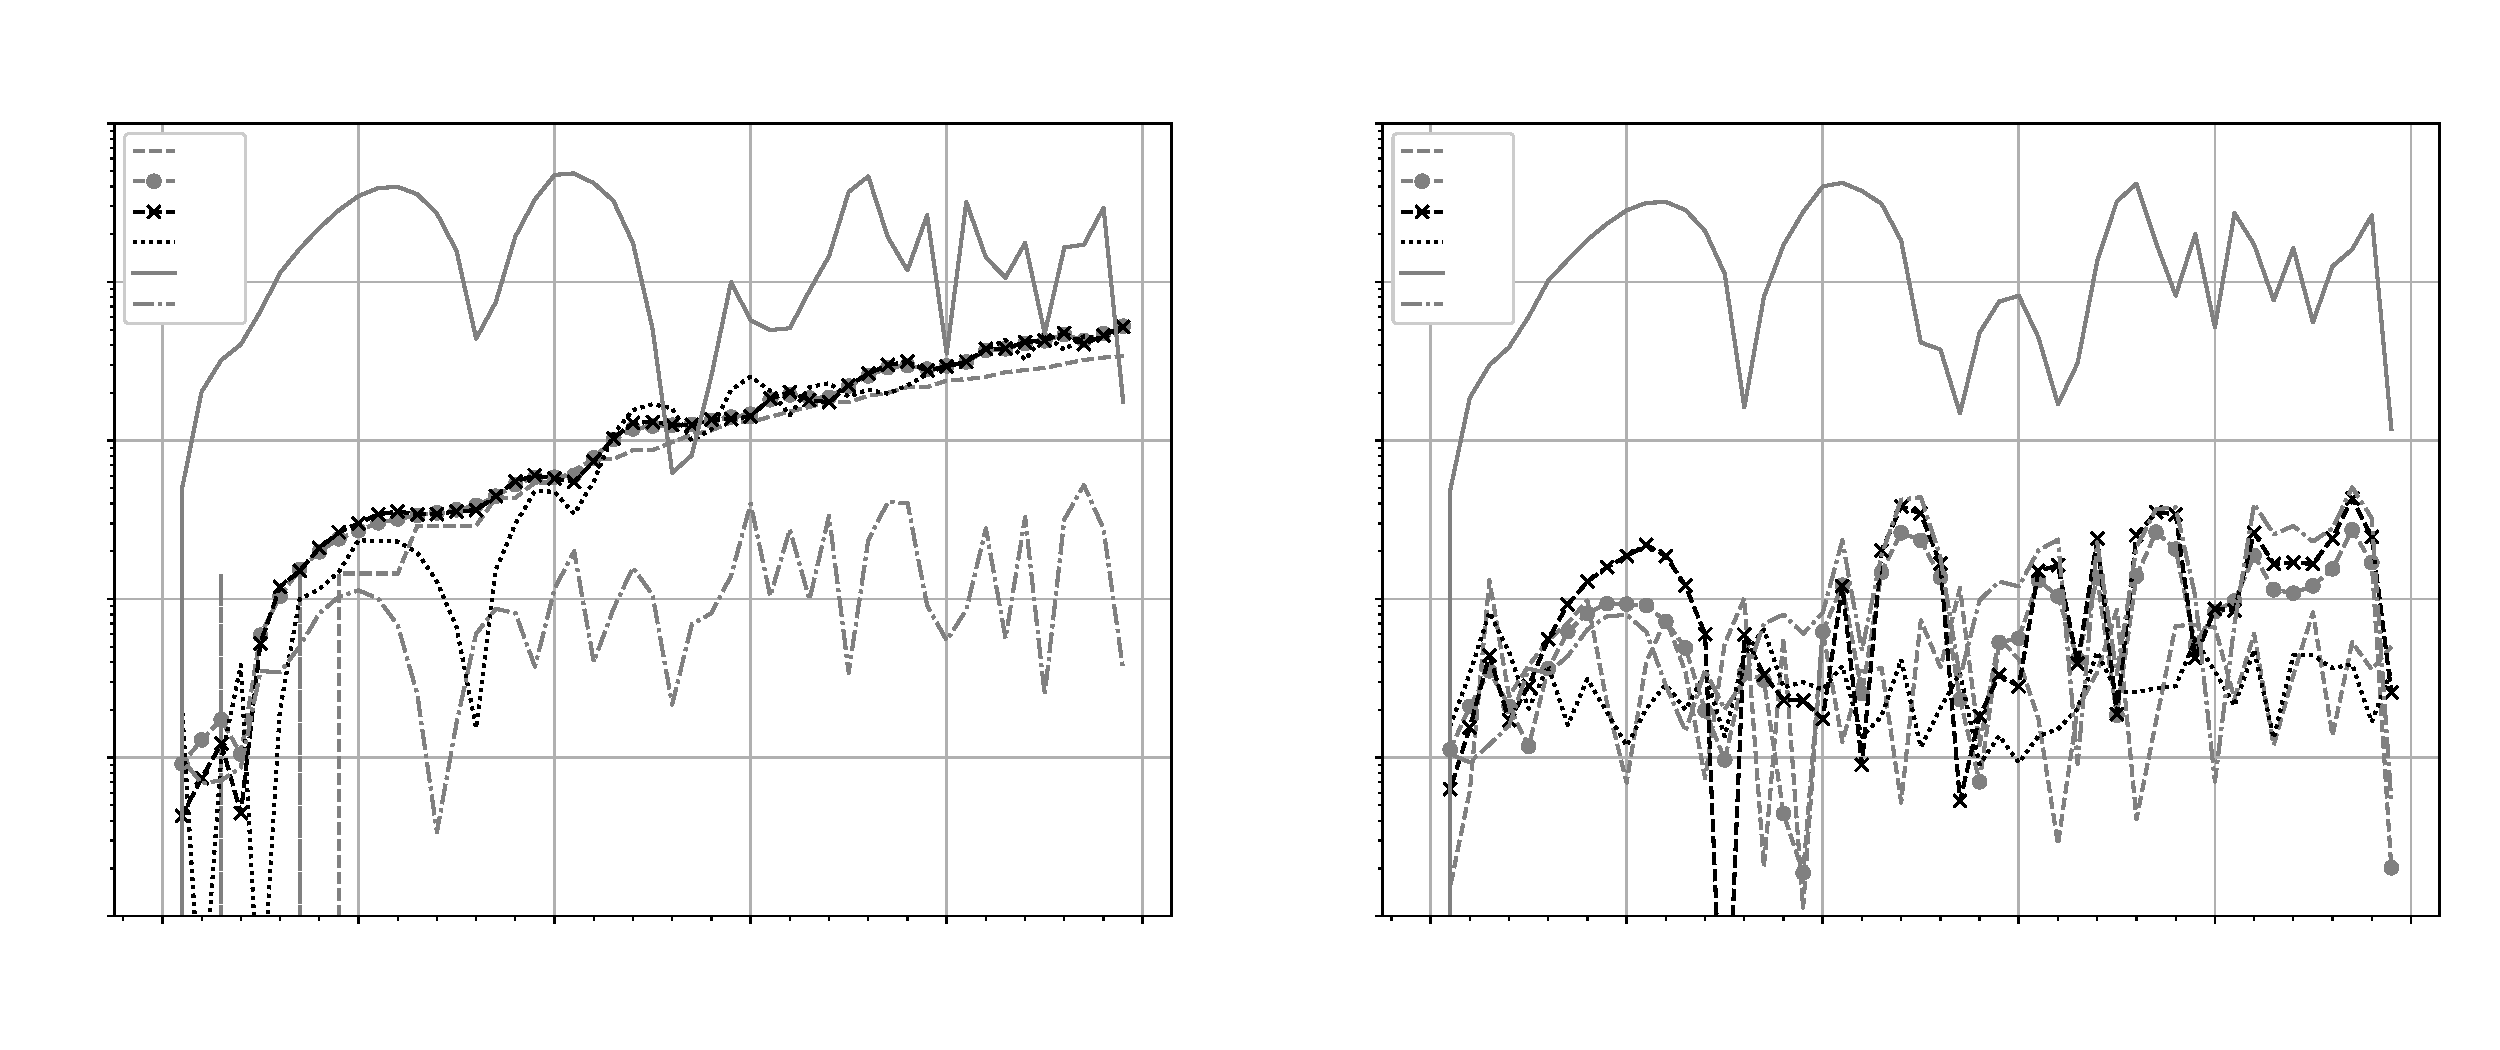
\includegraphics[width=\unitlength]{Rotsubrelerro.pdf}}%
    \put(0.06497309,0.04137704){\makebox(0,0)[b]{\smash{0}}}%
    \put(0.14340117,0.04137704){\makebox(0,0)[b]{\smash{10}}}%
    \put(0.22182923,0.04137704){\makebox(0,0)[b]{\smash{20}}}%
    \put(0.3002573,0.04137704){\makebox(0,0)[b]{\smash{30}}}%
    \put(0.37868536,0.04137704){\makebox(0,0)[b]{\smash{40}}}%
    \put(0.4571134,0.04137704){\makebox(0,0)[b]{\smash{50}}}%
    \put(0.25712184,0.02997863){\makebox(0,0)[b]{\smash{Angle (°)}}}%
    \put(0.02034155,0.0503764){\makebox(0,0)[lb]{\smash{10−2}}}%
    \put(0.02034155,0.1137964){\makebox(0,0)[lb]{\smash{10−1}}}%
    \put(0.02525822,0.1772164){\makebox(0,0)[lb]{\smash{100}}}%
    \put(0.02525822,0.2406364){\makebox(0,0)[lb]{\smash{101}}}%
    \put(0.02525822,0.3040564){\makebox(0,0)[lb]{\smash{102}}}%
    \put(0.02525822,0.3674764){\makebox(0,0)[lb]{\smash{103}}}%
    \put(0.01527515,0.21209243){\rotatebox{90}{\makebox(0,0)[b]{\smash{Relative Error (%)}}}}%
    \put(0.07659155,0.35681039){\makebox(0,0)[lb]{\smash{Rsm}}}%
    \put(0.07659155,0.34457862){\makebox(0,0)[lb]{\smash{Rq}}}%
    \put(0.07659155,0.33234685){\makebox(0,0)[lb]{\smash{Ra}}}%
    \put(0.07659155,0.32011506){\makebox(0,0)[lb]{\smash{Rt}}}%
    \put(0.07659155,0.3078833){\makebox(0,0)[lb]{\smash{Rsk}}}%
    \put(0.07659155,0.29565153){\makebox(0,0)[lb]{\smash{Rku}}}%
    \put(0.5722458,0.04137704){\makebox(0,0)[b]{\smash{0}}}%
    \put(0.65067389,0.04137704){\makebox(0,0)[b]{\smash{10}}}%
    \put(0.72910198,0.04137704){\makebox(0,0)[b]{\smash{20}}}%
    \put(0.80753007,0.04137704){\makebox(0,0)[b]{\smash{30}}}%
    \put(0.88595811,0.04137704){\makebox(0,0)[b]{\smash{40}}}%
    \put(0.96438615,0.04137704){\makebox(0,0)[b]{\smash{50}}}%
    \put(0.76439459,0.02997863){\makebox(0,0)[b]{\smash{Angle (°)}}}%
    \put(0.52761427,0.0503764){\makebox(0,0)[lb]{\smash{10−2}}}%
    \put(0.52761427,0.1137964){\makebox(0,0)[lb]{\smash{10−1}}}%
    \put(0.53253094,0.1772164){\makebox(0,0)[lb]{\smash{100}}}%
    \put(0.53253094,0.2406364){\makebox(0,0)[lb]{\smash{101}}}%
    \put(0.53253094,0.3040564){\makebox(0,0)[lb]{\smash{102}}}%
    \put(0.53253094,0.3674764){\makebox(0,0)[lb]{\smash{103}}}%
    \put(0.52254787,0.2120924){\rotatebox{90}{\makebox(0,0)[b]{\smash{Relative Error (%)}}}}%
    \put(0.5838643,0.35681039){\makebox(0,0)[lb]{\smash{Rsm}}}%
    \put(0.5838643,0.34457862){\makebox(0,0)[lb]{\smash{Rq}}}%
    \put(0.5838643,0.33234685){\makebox(0,0)[lb]{\smash{Ra}}}%
    \put(0.5838643,0.32011506){\makebox(0,0)[lb]{\smash{Rt}}}%
    \put(0.5838643,0.3078833){\makebox(0,0)[lb]{\smash{Rsk}}}%
    \put(0.5838643,0.29565153){\makebox(0,0)[lb]{\smash{Rku}}}%
  \end{picture}%
\endgroup%
